\let\oldlooseness=\looseness
\documentclass{csbulletin}
\selectlanguage{slovak}

\usepackage[utf8]{inputenc}
\usepackage[all]{nowidow}
\usepackage{lmodern}

\usepackage[backend=biber,style=iso-numeric,sortlocale=sk,autolang=other,bibencoding=UTF8,mincitenames=2,maxcitenames=2]{biblatex}
\addbibresource{references.bib}

\usepackage[implicit=false,hidelinks]{hyperref}
\usepackage{csquotes}

\usepackage{xcolor}
\usepackage{url}

\usepackage{xcolor}
\usepackage{listings}
\lstset{basicstyle=\ttfamily,
  showstringspaces=false,
  breaklines=true,
  columns=fullflexible
}

\usepackage{pifont}

\begin{document}

\selectlanguage{slovak}
\shorthandoff{-}

\title{Overleaf Community Edition: Postup inštalácie a~rozdiely oproti Overleaf Professional}
\EnglishTitle{Overleaf Community Edition: Installation and Comparison with Overleaf Professional}
\author{Michal Stano, Vít Starý Novotný}
\podpis{Michal Stano, astakus@mail.muni.cz\\Vít Starý Novotný, witiko@mail.muni.cz}
\maketitle[1ex]

\begin{abstract}
Webový editor Overleaf umožňuje pohodlné písanie dokumentov pomocou \LaTeX u. Veľkou výhodou Overleafu je, že umožňuje spoluprácu viacerých používateľov v~reálnom čase.
V tomto článku popíšeme postup inštalácie bezplatnej verzie Overleaf Community Edition na vlastné zariadenie a porovnáme ho s platenou verziou Overleaf Professional.
\end{abstract}
\klucoveslova: Overleaf, \LaTeX, Docker

\section{Úvod}
Vstup do sveta \TeX u bol pre prvého autora tohto článku náhly a~chaotický. V~druhom semestri štúdia na Fakulte informatiky Masarykovej univerzity si zapísal predmet \textit{Počítačové sítě -- cvičení}. Po každom cvičení dostali študenti za úlohu vypracovať protokol do šablóny v~\TeX u, k čomu im bol odporučený webový editor \emph{Overleaf}~\cite{novotny2021overleaf}. Keďže prvý autor o \TeX u vtedy ešte nič nevedel a~namiesto prečítania hocijakej príručky, manuálu alebo knihy sa rovno vrhol do práce, daný dokument dva dni štýlom pokus--omyl lepil dohromady z~kusov kódu z~rôznych fór, napr. StackExchange~\cite{stackexchange}, so značnou pomocou ChatGPT.

Prvého autora neskôr používanie \TeX u začalo baviť, ale kvôli jeho štýlu písania ,,napíšem, skompilujem a~uvidím`` stále preferoval Overleaf oproti manuálnej kompilácii. Preto ho neskôr prekvapilo, keď Overleaf zrazu jeho dokument skompilovať nechcel. Používal totižto bezplatnú verziu \textit{Overleaf Free}. Nevedel, či bol jeho projekt len priveľký, alebo sa musel kompilovať niekoľkokrát, ale podarilo sa mu prekonať \href{https://www.overleaf.com/learn/how-to/Overleaf_plan_limits}{časový limit kompilácie}.

Overleafu sa vzdať nechcel, a~tak rýchlo hľadal spôsob, ako časový limit a~kompilačnú kapacitu Overleafu navýšiť.
Okrem platenej verzie \href{https://www.overleaf.com/user/subscription/plans}{\textit{Premium}} vo variantoch \textit{Standard} a~\textit{Professional} (ďalej len \textit{Overleaf~Pro}), bola ešte možnosť stiahnuť si software~\textit{Overleaf Toolkit} a~Overleaf prevádzkovať lokálne na vlastnom zariadení alebo serveri. Overleaf Toolkit je dostupný vo dvoch verziách, \textit{Community Edition} a~\textit{Enterprise}. Community Edition (ďalej len \textit{Overleaf~CE}) je dostupná zadarmo, ale bez profesionálnej podpory, zatiaľ čo Enterprise je platená, určená najmä pre velké (napr. firemné) serveri a~s~profesionálnou podporou. Zvolil si preto Overleaf~CE, keďže Overleaf chcel len na vlastné použitie. Proces inštalácie vyzeral jednoducho, a~tak sa do toho pustil.

\section{Príprava systému}
Pred samotnou inštaláciou je potrebné si pár vecí pripraviť. Keďže prvž autor použil Linux Mint, ktorý vychádza z~Ubuntu a~teda Debianu, popíšeme postup prispôsobený pre Debianové distribúcie Linuxu. Ak niektorý príkaz zlyhá s~výstupom ,,\foreignlanguage{english}{permission denied}``, treba pred daný príkaz napísať \lstinline{sudo}.

Na inštaláciu a~fungovanie Overleafu je potrebné mať nainštalované \textit{Bash} a~\textit{Docker}. Neskôr pri inštalácií \TeX u je potrebný aj \textit{Perl}.

Docker môžeme nainštalovať nasledujúcimi príkazmi:
\begin{lstlisting}
$ apt update
$ apt install docker docker.io docker-compose-v2
\end{lstlisting}
%   \texttt{Docker-compose} je od polovice tohto roku zastaralý, oficiálne bez podpory a~nahradený Docker compose V2~\cite{compose}. Spolu s V2 by sa mal automaticky stiahnuť aj \texttt{Docker.io}, ak sa ale nestiahne, je potrebné stiahnuť aj ten.
%
Ak by neskôr počas inštalácie Docker písal ,,\foreignlanguage{english}{cannot connect to the Docker daemon}``, je potrebné zadať nasledujúci príkaz:
\begin{lstlisting}
$ systemctl start docker
\end{lstlisting}

Bash a~Perl sa na Linuxe väčšinou nacházdajú natívne.

\section{Inštalácia Overleafu~CE}
Overleaf~CE nainštalujeme postupom vysvetleným v oddieli \href{https://github.com/overleaf/toolkit}{\textit{Installation}} súboru \texttt{README.md} v~Git repozitári Overleaf-toolkit~\cite{overleaf_git}.

Najprv si do vybratého priečinku stiahneme súbory z~vyššie spomenutého úložiska a~po stiahnutí vstúpime do vytvoreného priečinku:
\begin{lstlisting}
$ git clone https://github.com/overleaf/toolkit ./overleaf-toolkit
$ cd overleaf-toolkit/
\end{lstlisting}
Každý príkaz odteraz vychádza z~toho, že pracujeme v~tomto priečinku.

Konfiguráciu vytvoríme príkazom \lstinline{$ bin/init}, ktorý v~priečinku \texttt{config} vytvorí súbory \texttt{overleaf.rc}, \texttt{variables.env} a~\texttt{version}.
V~prípade, že chceme povoliť prístup z~iných zariadení, napríklad v~prípade používania serveru na hosťovanie Overleafu, v~súbore \texttt{overleaf.rc} je treba pomocou textového editoru priamo v~termináli, napr. Vim alebo Nano, hodnotu \texttt{SHARELATEX\_LISTEN\_IP} prestaviť zo~127.0.0.1 na 0.0.0.0 alebo na IP adresu konkrétneho sieťového rozhrania.

Ostáva Overleaf spustiť jedným z dvoch nasledujúcich príkazov:
\begin{lstlisting}
$ bin/up
$ bin/start
\end{lstlisting}
Tieto príkazy sú vo výsledku rovnaké, majú len jeden menší rozdiel, ktorý hneď popíšeme. Oba však na pozadí odkazujú na sériu skriptov, ktoré pre nás automaticky spustia celý Overleaf systém, t.~j. postarajú sa o spustenie \texttt{Docker Compose}, ktorý spravuje 3 docker kontajnery: \textit{redis}, \textit{mongo} a~\textit{sharelatex}.

Pri použití príkazu \lstinline{$ bin/up} sa terminál, alebo jeho inštancia, na ktorej bol príkaz spustený, prepojí so záznamom výstupu. Preto je odporúčané prvýkrát použiť tento príkaz, keďže je priamo v~termináli vidieť, čo sa so systémom deje. Nevýhodou tohto príkazu je zablokovanie daného terminálu pre ďalšie použitie až do zastavenia procesu. Vypnúť kontajnery (a odblokovať daný terminál) sa dá len pomocou klávesovej skratky~\verb|CTRL + C|.

Príkaz \lstinline{$ bin/start} spustí kontajnery, na terminál vypíše stav jednotlivých kontajnerov (napr.: \ding{51} \lstinline{Container sharelatex Started}), ale inak nechá terminál tak. Vypnúť sa dá príkazom \lstinline{$ bin/stop}.

Ak sa služba spustila bez problémov, t.~j. výpis príkazu \lstinline{$ bin/up} neobsahuje chyby, alebo~všetky kontajnery majú vo výpise príkazu \lstinline{$ bin/start} status ,,Started`` alebo ,,Healthy``, Overleaf funguje.
Pred začiatkom práce môžeme ešte aktualizovať distribúciu \TeX~Live~\cite{texlive} v~kontajneri sharelatex následne:
\begin{lstlisting}
$ bin/shell
# tlmgr update --self --all
\end{lstlisting}

\vspace*{-1em}
\section{Účet administrátora, prihlásenie a~prvý projekt}
\vspace*{-0.5em}

Na vytvorenie prvého projektu stačí vytvoriť účet administrátora a~prihlásiť sa.

Vo~webovom prehliadači na adrese \href{http://localhost/launchpad}{\lstinline{http://localhost/launchpad}} vyplníme do kolóniek ,,email`` a~,,heslo`` prihlasovacie údaje administrátora a následne sa na adrese~\url{http://localhost/login} prihlásime pomocou týchto prihlasovacích údajov. Po prihlásení budeme automaticky presmerovaní na adresu \url{http://localhost/project} so zoznamom všetkých projektov. Na obrázku~\ref{fig:example-project} je zobrazený ukážkový projekt, ktorý je distribuovaný spolu s Overleafom~CE.

\begin{figure}[b!]
    \vspace*{-0.5em}
    \centering
    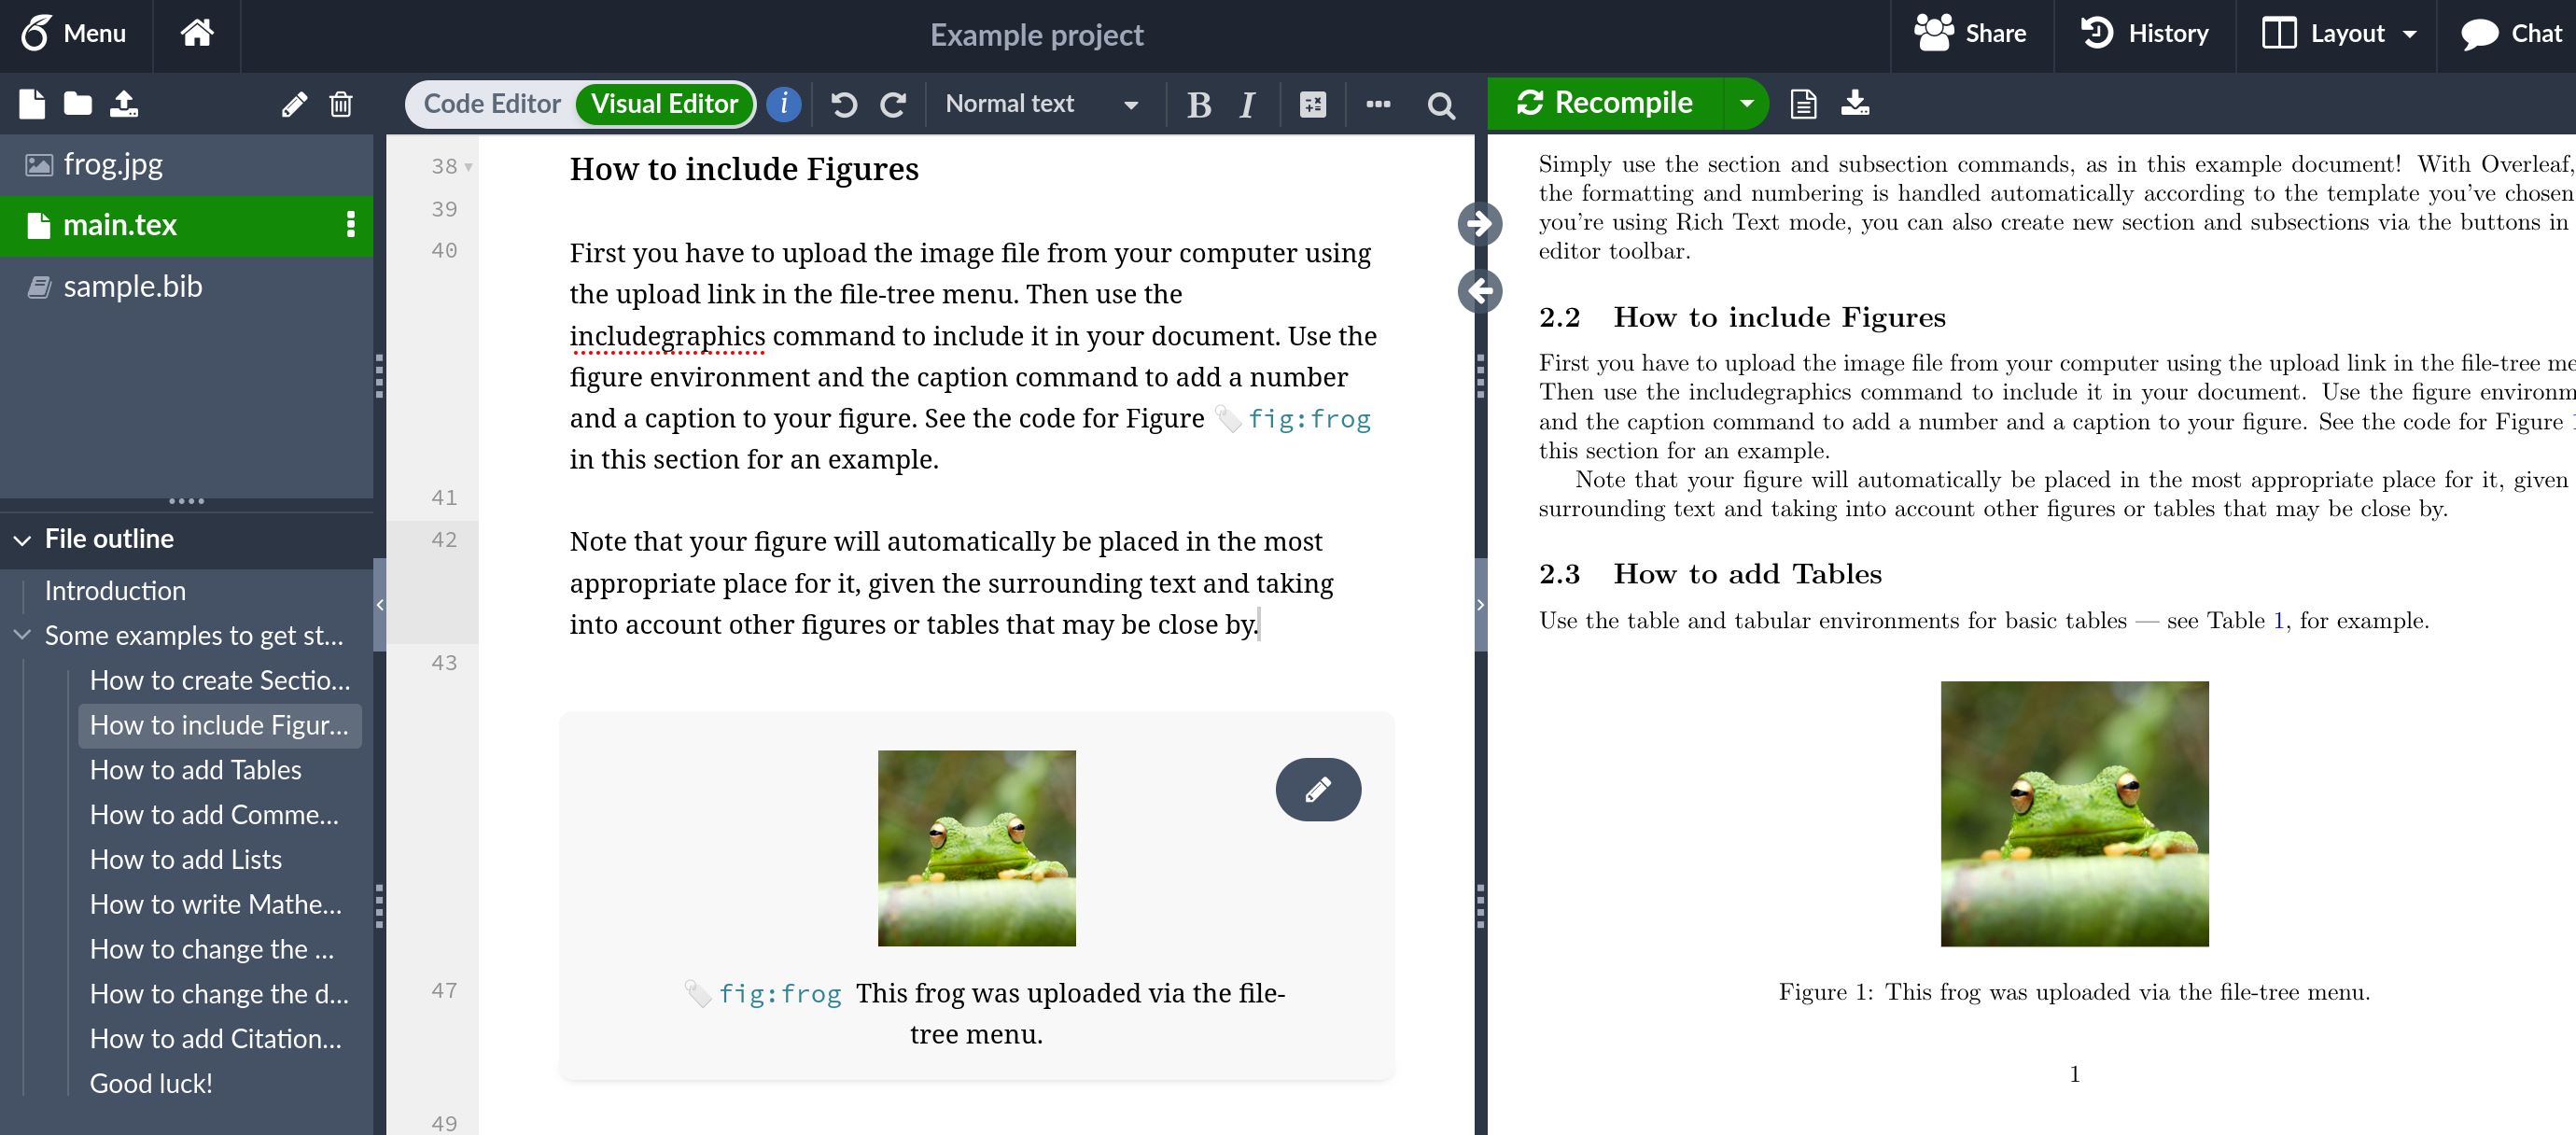
\includegraphics[width=\textwidth]{example-project}
    \par
    \vspace*{-0.5em}
    \caption{Ukážkový projekt v~Overleafe CE}
    \label{fig:example-project}
\end{figure}

\iffalse

\section{Inštalácia \TeX u}
% VSN: TeX Live je již instalovaný v kontejneru sharelatex, není třeba ho instalovat znovu.
Overleaf už funguje a~môžeme vytvoriť náš prvý projekt, ale pred prekladom nášho dokumentu musíme ešte nainštalovať \TeX.

Pri inštalácií som postupoval podľa inštrukcií na stránke distribúcie \TeX~Live~\cite{texlive}. Na to som sa musel dostať do shellu v~Dockeri príkazom \lstinline{$ bin/shell}. V~prostredí kontajneru som stiahol inštalátor \TeX~Live, archív rozbalil a~spustil inštalácii:
\begin{lstlisting}
$ wget mirror.ctan.org/systems/texlive/tlnet/install-tl-unx.tar.gz
$ tar xf install-tl-unx.tar.gz
$ cd install-tl-*/
$ perl install-tl
\end{lstlisting}

Počas procesu sa nás skript opýta, či chceme použiť predošlú konfiguráciu. Keďže bez predošlého importovania žiadnu konfigurácie nemáme, je bezpečné to ignorovať a~pokračovať ďalej. V~momente keď sa objavil výpis ,,enter command``, postupne som použil možnosti \texttt{O/o} (\foreignlanguage{english}{Options}), \texttt{L/l} (\foreignlanguage{english}{Create symlinks in standard directories}), \texttt{R/r} (\foreignlanguage{english}{Return to main menu}) a~\texttt{I/i} (\foreignlanguage{english}{Start installation to hard disk}).

Skript inštaluje viac ako 4000 balíkov, takže to nejaký čas potrvá (na mojom laptope to trvalo skoro hodinu).

\fi

\vspace*{-2.5em}
\section{Porovnanie Overleafu~CE a Overleafu~Pro}
\vspace*{-0.5em}
Neskôr počas semestru sa prvý autor dozvedel, že ako študent Fakulty informatiky Masarykovej univerzity má možnosť aktivovať si zadarmo Overleaf Pro. Po aktivácii účtu sa rozhodol, že Overleaf~Pro a Overleaf~CE porovná.

\begin{figure}[t]
    \centering
    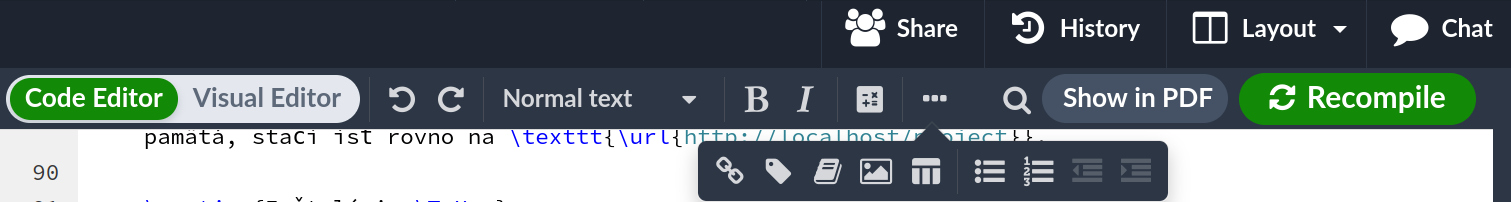
\includegraphics[width=\textwidth]{ui-ce}
    \par
    \smallskip
    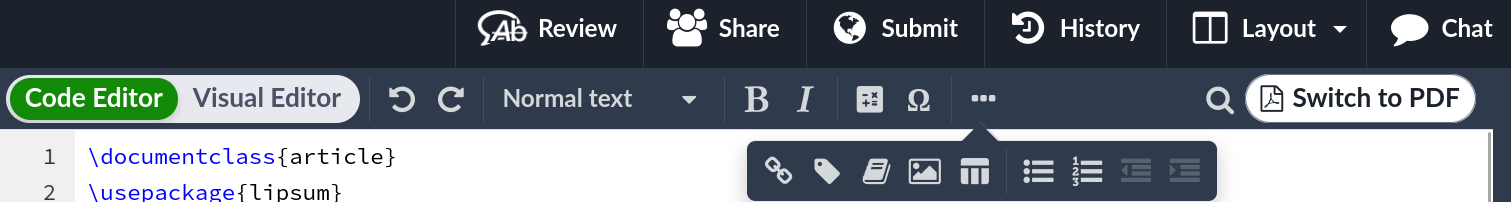
\includegraphics[width=\textwidth]{ui-pro}
    \par
    \vspace*{-0.5em}
    \caption{Rozhranie Overleafu~CE (hore) a~Overleafu~Pro (dole)}
    \label{fig:ui-differences}
\end{figure}

\vspace*{-0.5em}
\subsection{Používateľské rozhranie}
Veľké rozdiely medzi Overleafmi~CE a Pro sme nezaregistrovali až na pár zmien v~užívateľskom rozhraní, pozrite obrázok~\ref{fig:ui-differences}.

V~Overleaf~Pro sú pridané tlačidlá ,,Publish``, ktorými je možné projekt zverejniť na preprintových archívoch, alebo ho ponúknuť na vydanie partnerským vydavateľstvám, a~,,Review``, ktoré umožňuje zobraziť komentáre a~navrhované zmeny od korektora a spoluautorov. Taktiež je v hornej lište pridané tlačidlo $\Omega$, ktoré otvorí knižnicu symbolov a špeciálnych znakov. V~Overleafe~CE tieto funkcie nie sú z viacerých dôvodov. ,,Publish`` a ,,Review`` nie sú zahrnuté kvôli tomu, že sme izolovaní od serveru Overleaf. Špeciálne znaky sú súčasťou výhod verzie Premium a teda sú nedostupné v Overleafe~CE ako aj vo verzii Free.

Až na pár drobností je aj samotný textový editor rovnaký. Jediné, čo by prvý autor tvorcom vytkol je, že Overleaf~CE pri príkaze \verb|\cite{}| alebo \verb|\includesvg{}| nedopĺňa kľúč. Zaujímavé je, že po \verb|\includegraphics{}| ich dopĺňa.

\begin{figure}[t]
    \centering
    
\includegraphics[width=\textwidth]{collaboration}
    \par
    \vspace*{-0.5em}
    \caption{Spolupráca dvoch používateľov v~Overleafe~CE}
    \label{fig:collaboration}
\end{figure}

\vspace*{-0.5em}
\subsection{Kolaboratívna spolupráca}
V Overleafe~CE môžeme na projektoch spolupracovať s ďalšími používateľmi podobne ako v~Overleafe~Pro. Najprv by sme z administrátorského účtu na adrese~\url{http://localhost/admin/register} vytvorili nové používateľské účty. Následne by sme do projektu cez tlačidlo ,,\foreignlanguage{english}{Share}`` pozvali ďalších používateľov. Títo používatelia potom môžu na projekte pracovať súbežne, pozrite obrázok~\ref{fig:collaboration}.

\section{Záver}

Webový editor Overleaf~\cite{novotny2021overleaf} umožňuje pohodlné písanie dokumentov pomocou \LaTeX u. V tomto článku sme ukázali, ako môžeme nainštalovať bezplatnú self-hosted verziu Overleaf CE na vlastný laptop alebo firemný server, vytvárať projekty a spolupracovať na nich s~ďalšími používateľmi. Sme presvedčení, že pre mnohých užívateľov je Overleaf CE zaujímavou alternatívou oproti cloudovým verziám Overleafu, ktorá umožňuje používať na sadzbu \LaTeX ových dokumentov vlastný hardware a vyhnúť sa obmedzeniam verzie Overleaf Free.

\printbibliography  

\begin{summary}
The Overleaf web editor enables convenient writing of documents using \LaTeX. A significant advantage of Overleaf is that it enables collaboration among multiple users in real-time. In this article, we describe the process of installing the free version of Overleaf Community Edition on your own device and compare it with the paid version of Overleaf Professional.
\keywords: Overleaf, \LaTeX, Docker
\end{summary}
\end{document}
